%
% $RCSfile: architectural.tex,v $
%
% Copyright (C) 2002-2008. Christian Heller.
%
% Permission is granted to copy, distribute and/or modify this document
% under the terms of the GNU Free Documentation License, Version 1.1 or
% any later version published by the Free Software Foundation; with no
% Invariant Sections, with no Front-Cover Texts and with no Back-Cover
% Texts. A copy of the license is included in the section entitled
% "GNU Free Documentation License".
%
% http://www.cybop.net
% - Cybernetics Oriented Programming -
%
% http://www.resmedicinae.org
% - Information in Medicine -
%
% Version: $Revision: 1.1 $ $Date: 2008-08-19 20:41:05 $ $Author: christian $
% Authors: Christian Heller <christian.heller@tuxtax.de>
%

\subsection{Architectural}
\label{architectural_heading}
\index{Architectural Pattern}

\emph{Architectural Patterns} are templates for the gross design of software
systems. They describe concrete software architectures and provide basic
structuring (modularisation) principles.

%
% $RCSfile: layers.tex,v $
%
% Copyright (C) 2002-2008. Christian Heller.
%
% Permission is granted to copy, distribute and/or modify this document
% under the terms of the GNU Free Documentation License, Version 1.1 or
% any later version published by the Free Software Foundation; with no
% Invariant Sections, with no Front-Cover Texts and with no Back-Cover
% Texts. A copy of the license is included in the section entitled
% "GNU Free Documentation License".
%
% http://www.cybop.net
% - Cybernetics Oriented Programming -
%
% http://www.resmedicinae.org
% - Information in Medicine -
%
% Version: $Revision: 1.1 $ $Date: 2008-08-19 20:41:07 $ $Author: christian $
% Authors: Christian Heller <christian.heller@tuxtax.de>
%

\subsubsection{Layers}
\label{layers_heading}
\index{Layers Pattern}
\index{Presentation Layer}
\index{Domain Logic Layer}
\index{Business Logic Layer}
\index{Data Source Layer}
\index{ISO OSI Model Layers}
\index{Relaxed Layered System}

The \emph{Layers} pattern \cite{buschmann} is one of the most often used
principles to subdivide a system into logical levels. One variant was shown in
figure \ref{logical_figure}, at the beginning of this chapter. It contained the
three layers \emph{Presentation}, \emph{Domain Logic} and \emph{Data Source}. A
more general illustration can be seen in figure \ref{layers_figure}. It shows a
client using the functionality encapsulated in a layer. That top-most layer
delegates subtasks to lower-level layers which are specialised on solving them.
Another well-known example making use of this pattern is the \emph{ISO OSI}
model as introduced in section \ref{systems_interconnection_heading}.

\begin{figure}[ht]
    \begin{center}
        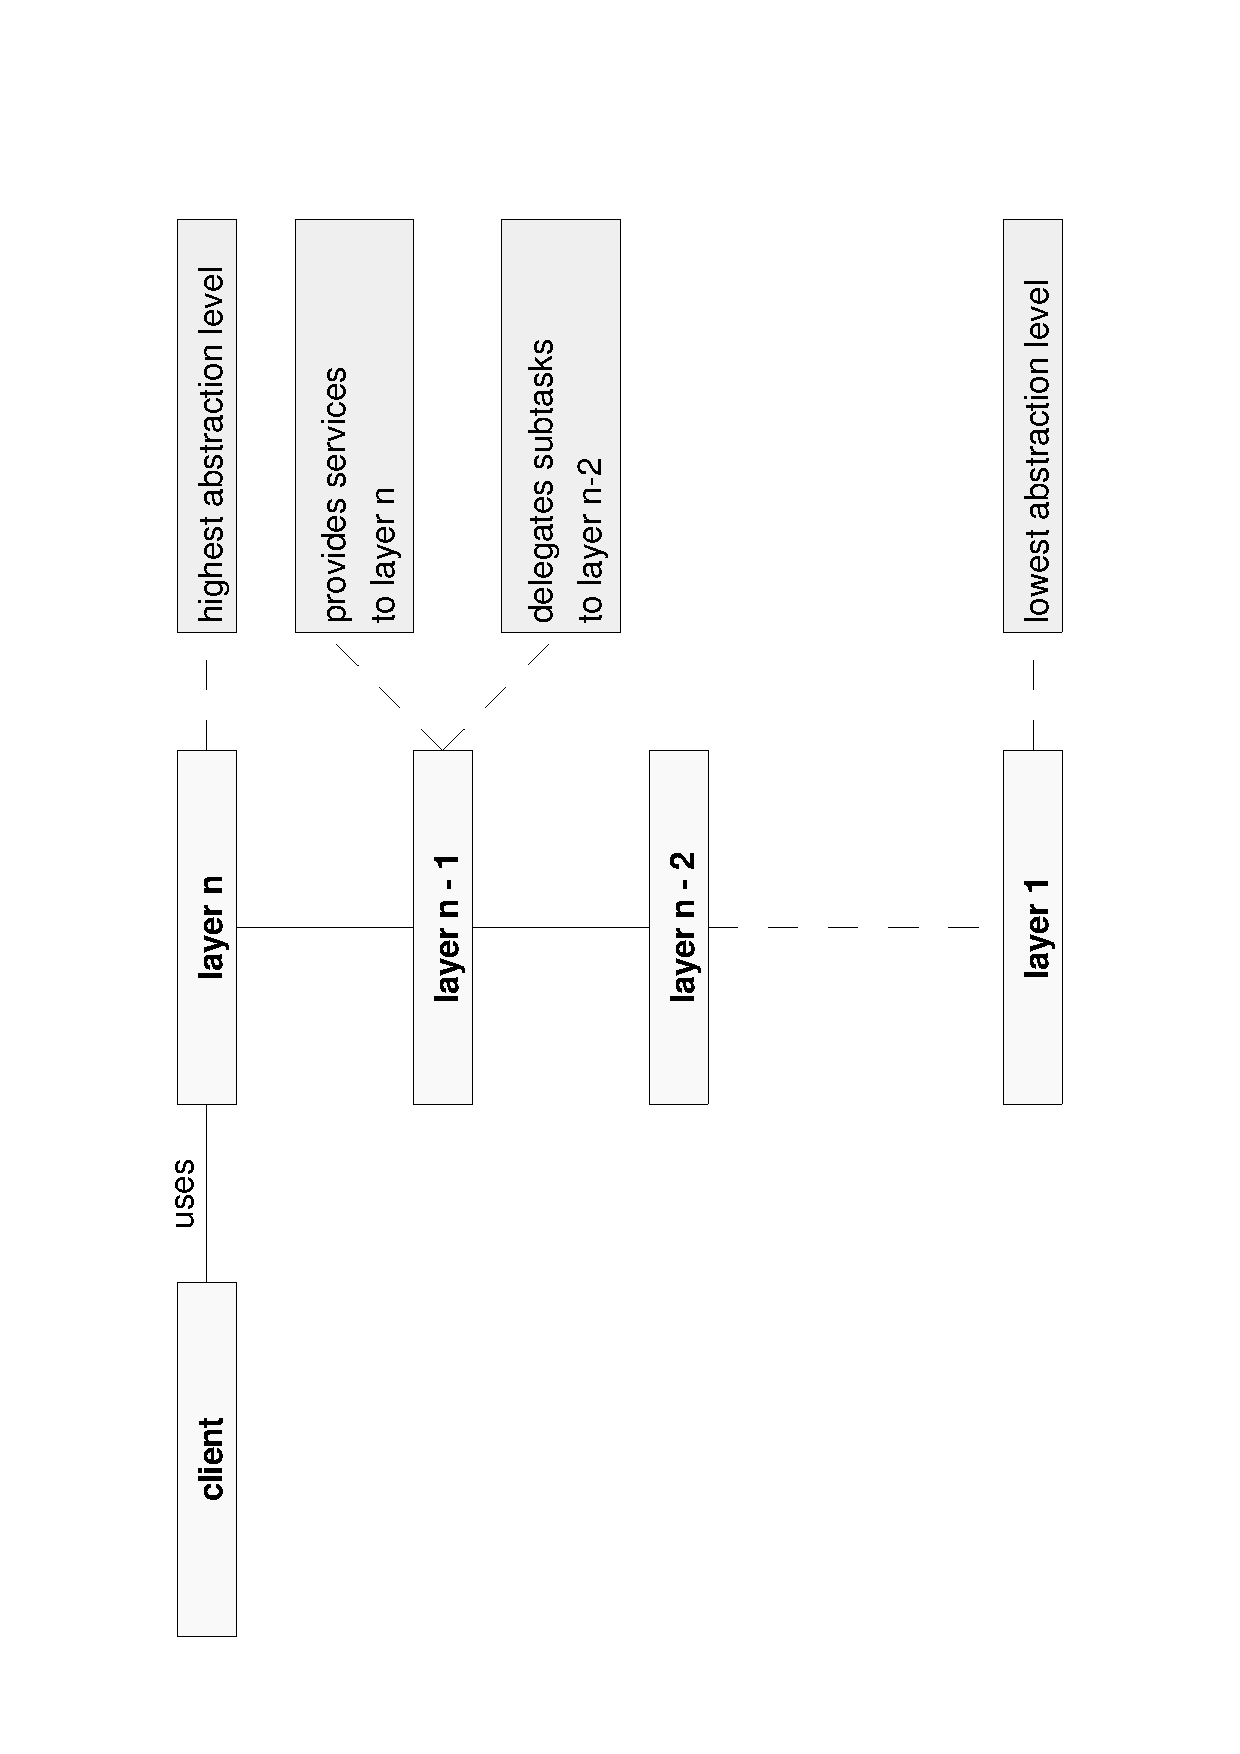
\includegraphics[scale=0.3,angle=-90]{graphic/layers.pdf}
        \caption{Layers Pattern}
        \label{layers_figure}
    \end{center}
\end{figure}

One variant of this pattern, mentioned by Buschmann \cite{buschmann}, is the
\emph{Relaxed-Layered-System}. It permits a layer to not only use the services
of its direct base layer, but also of yet lower-situated layers. The base layer,
in this case, is called \emph{transparent}.

The ontology examples in chapter \ref{knowledge_schema_heading} are organised
according to the \emph{Layers} pattern. Their layers represent levels of
growing granularity.

%
% $RCSfile: layer_supertype.tex,v $
%
% Copyright (C) 2002-2008. Christian Heller.
%
% Permission is granted to copy, distribute and/or modify this document
% under the terms of the GNU Free Documentation License, Version 1.1 or
% any later version published by the Free Software Foundation; with no
% Invariant Sections, with no Front-Cover Texts and with no Back-Cover
% Texts. A copy of the license is included in the section entitled
% "GNU Free Documentation License".
%
% http://www.cybop.net
% - Cybernetics Oriented Programming -
%
% http://www.resmedicinae.org
% - Information in Medicine -
%
% Version: $Revision: 1.1 $ $Date: 2008-08-19 20:41:07 $ $Author: christian $
% Authors: Christian Heller <christian.heller@tuxtax.de>
%

\subsubsection{Layer Supertype}
\label{layer_supertype_heading}
\index{Layer Supertype Pattern}

The \emph{Layer Supertype} pattern \cite{fowler2002} is a rather simple but
quite useful one. It assumes that a system is structured using the
\emph{Layers} pattern. What the pattern proposes is to add a (possibly
abstract) class that all other classes in its layer inherit from (figure
\ref{supertype_figure}). The reason is that basic functionality common to all
classes in a layer, for example persistence- or logging capabilities, can be
provided once by the supertype, such avoiding redundancies.

\begin{figure}[ht]
    \begin{center}
        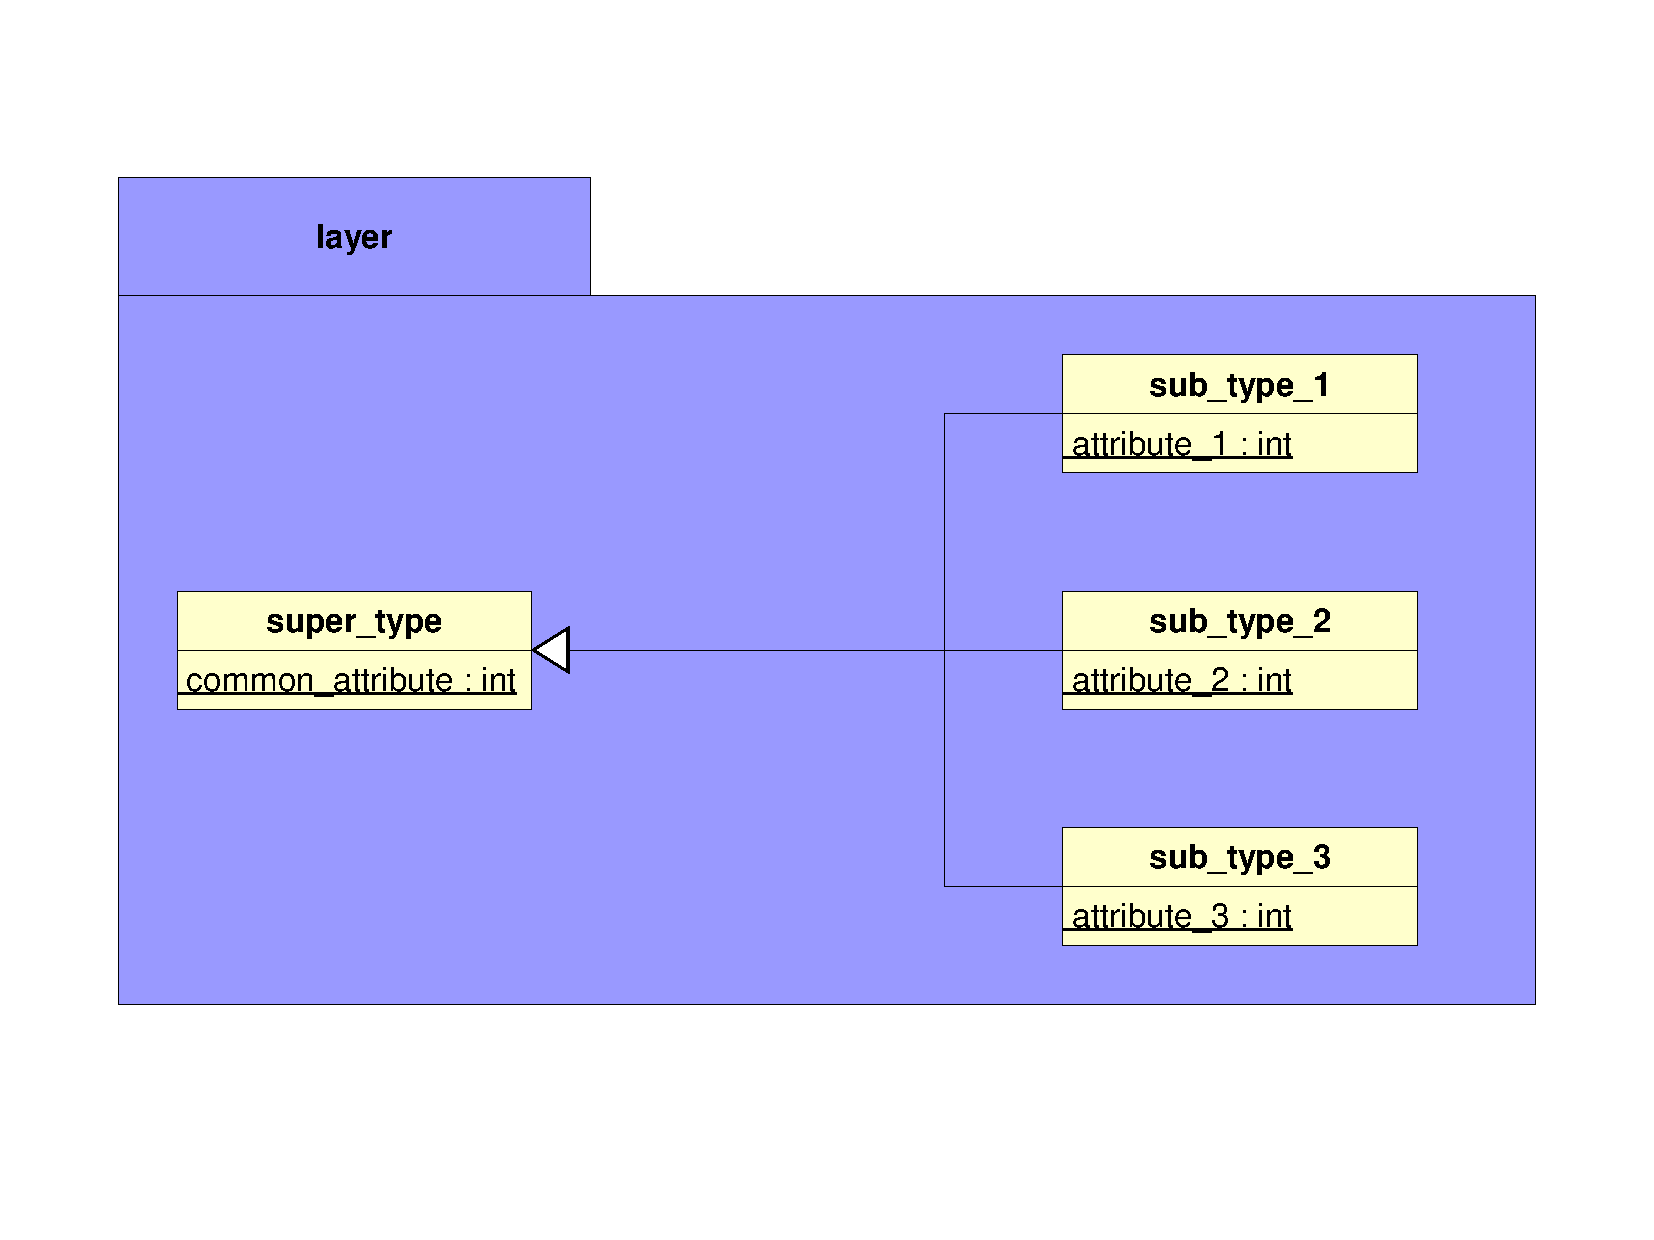
\includegraphics[scale=0.3,angle=-90]{graphic/supertype.pdf}
        \caption{Layer Supertype Pattern}
        \label{supertype_figure}
    \end{center}
\end{figure}

The language introduced in chapter \ref{cybernetics_oriented_language_heading}
does not use inheritance and thus cannot use super knowledge templates in the
meaning of the \emph{Layer Supertype} pattern. Nevertheless, the pattern is important
because of its idea to categorise similar knowledge, such as all templates of:
a \emph{Textual User Interface} (TUI), a \emph{Graphical User Interface} (GUI),
a \emph{Domain Model} etc.

%
% $RCSfile: domain_model.tex,v $
%
% Copyright (C) 2002-2008. Christian Heller.
%
% Permission is granted to copy, distribute and/or modify this document
% under the terms of the GNU Free Documentation License, Version 1.1 or
% any later version published by the Free Software Foundation; with no
% Invariant Sections, with no Front-Cover Texts and with no Back-Cover
% Texts. A copy of the license is included in the section entitled
% "GNU Free Documentation License".
%
% http://www.cybop.net
% - Cybernetics Oriented Programming -
%
% http://www.resmedicinae.org
% - Information in Medicine -
%
% Version: $Revision: 1.1 $ $Date: 2008-08-19 20:41:06 $ $Author: christian $
% Authors: Christian Heller <christian.heller@tuxtax.de>
%

\subsubsection{Domain Model}
\label{domain_model_heading}
\index{Domain Model Pattern}

One of the three layers in figure \ref{logical_figure} shown at the beginning
of this chapter is the \emph{Domain Model}. Fowler \cite{fowler2002} proposed
it as singular pattern because of its importance in large-scale business
systems. Figure \ref{domainmodel_figure} shows an imaginary business domain
model. The actual focus, however, should not be put on the inside structure of
this example model, but on the fact that the domain model represents a layer on
its own.

\begin{figure}[ht]
    \begin{center}
        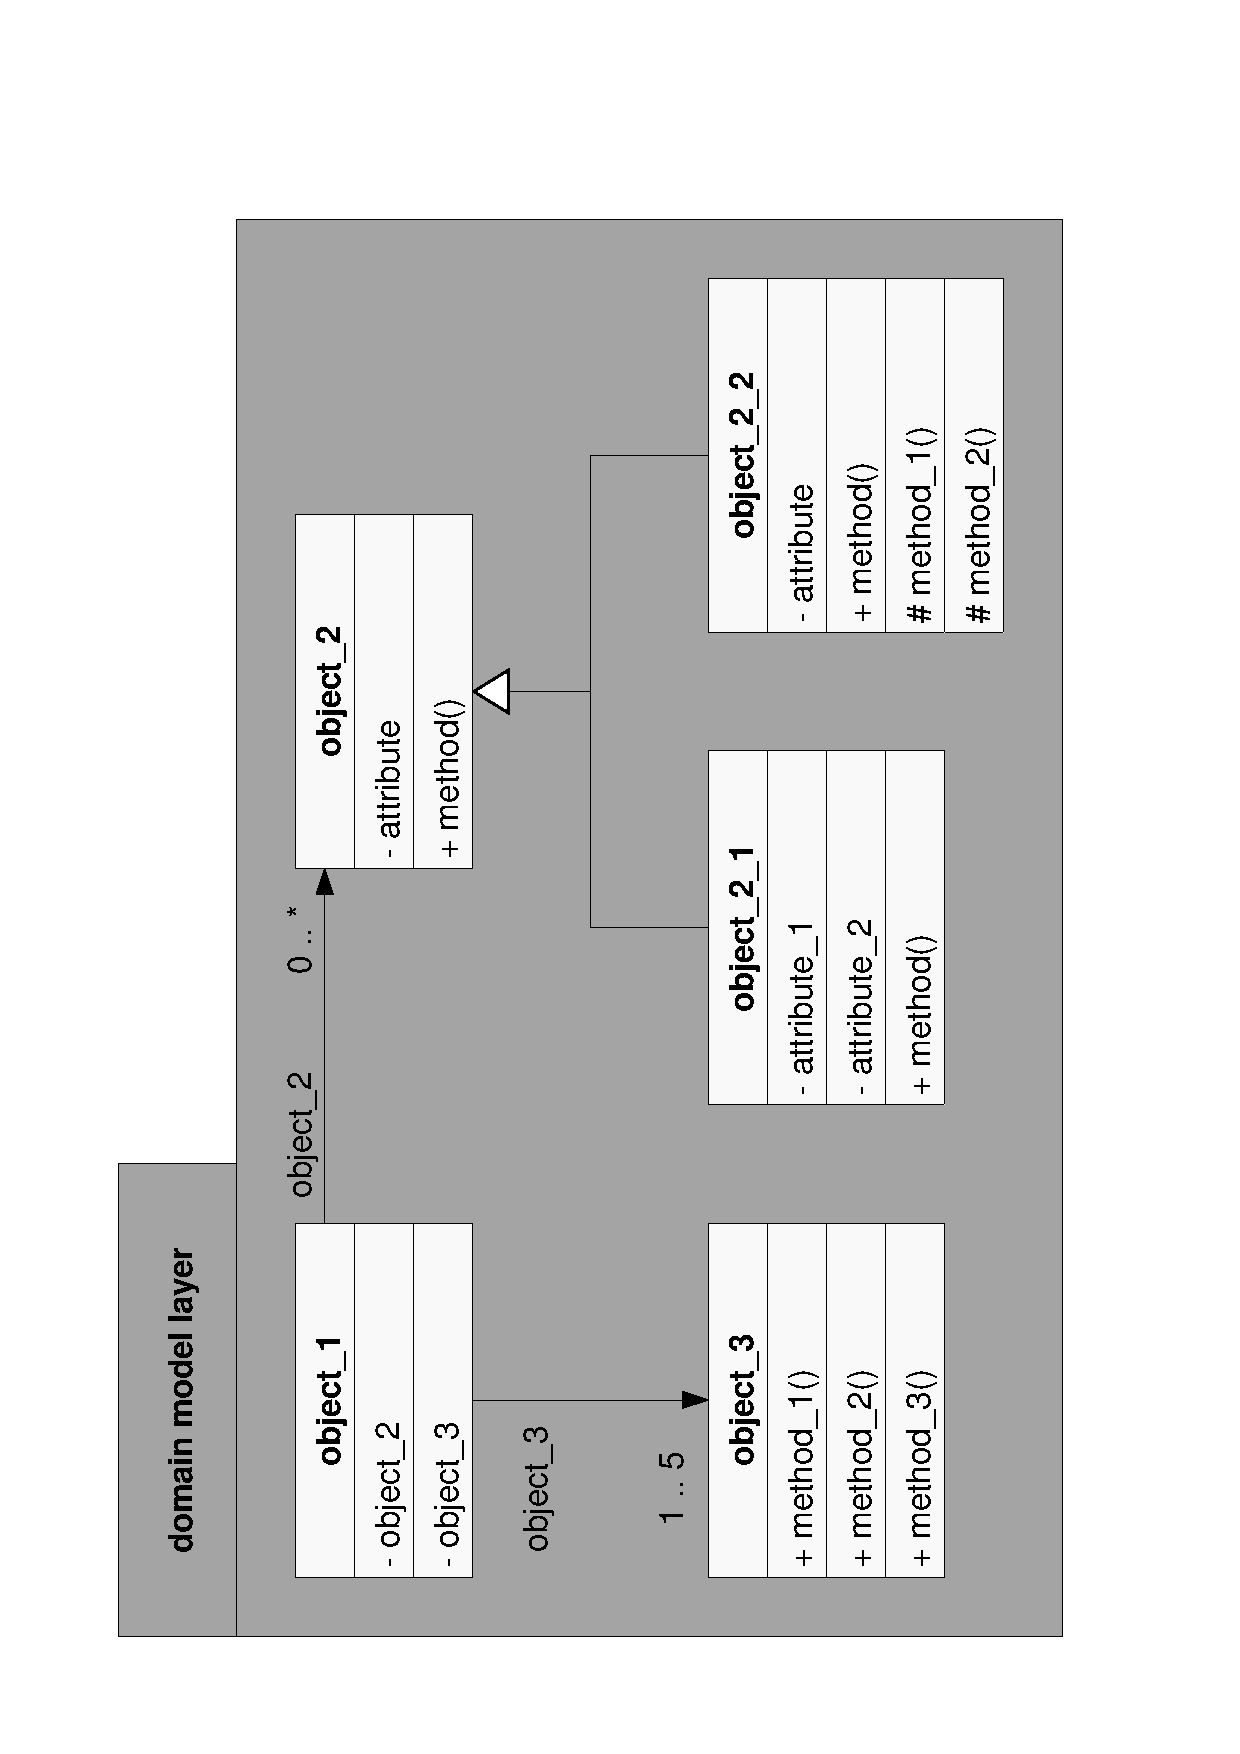
\includegraphics[scale=0.3,angle=-90]{graphic/domainmodel.pdf}
        \caption{Domain Model Pattern}
        \label{domainmodel_figure}
    \end{center}
\end{figure}

This separation cannot be found in all systems and in fact, it does not make
sense for \emph{all} systems. Small solutions let their user interface or
application control, respectively, access a database directly which avoids the
rather big effort of creating a special domain model. But the larger the system
to be created and the more clear the desired architecture shall be, the more
recommendable it is to use the \emph{Domain Model} pattern.

It will be helpful to have heard about this pattern when reading chapter
\ref{state_and_logic_heading} dealing with domain-, user interface- and other
models and their translation into each other.

%
% $RCSfile: data_mapper.tex,v $
%
% Copyright (c) 2004. Christian Heller. All rights reserved.
%
% No copying, altering, distribution or any other actions concerning this
% document, except after explicit permission by the author!
% At some later point in time, this document is planned to be put under
% the GNU FDL license. For now, _everything_ is _restricted_ by the author.
%
% http://www.cybop.net
% - Cybernetics Oriented Programming -
%
% http://www.resmedicinae.org
% - Information in Medicine -
%
% @author Christian Heller <christian.heller@tuxtax.de>
%

\paragraph{Data Mapper}
\label{data_mapper_heading}

Besides the \emph{Domain Logic}, standard three-tier architectures contain a
\emph{Data Source} layer which may for example represent a database. Both layers
need to exchange data. Modern systems use OOP methods to implement the domain
model. Database models, on the other hand, are often implemented as
\emph{Entity Relationship Model} (ERM).

In order to avoid close coupling and a mix-up of both layers, the introduction
of an additional \emph{Data Mapper} layer \cite{fowler2002} in between the two
others may be justified (figure \ref{datamapper_figure}). The most important
idea of this pattern is to abolish the interdependencies of domain- and
persistence model (database).

\begin{figure}[ht]
    \begin{center}
        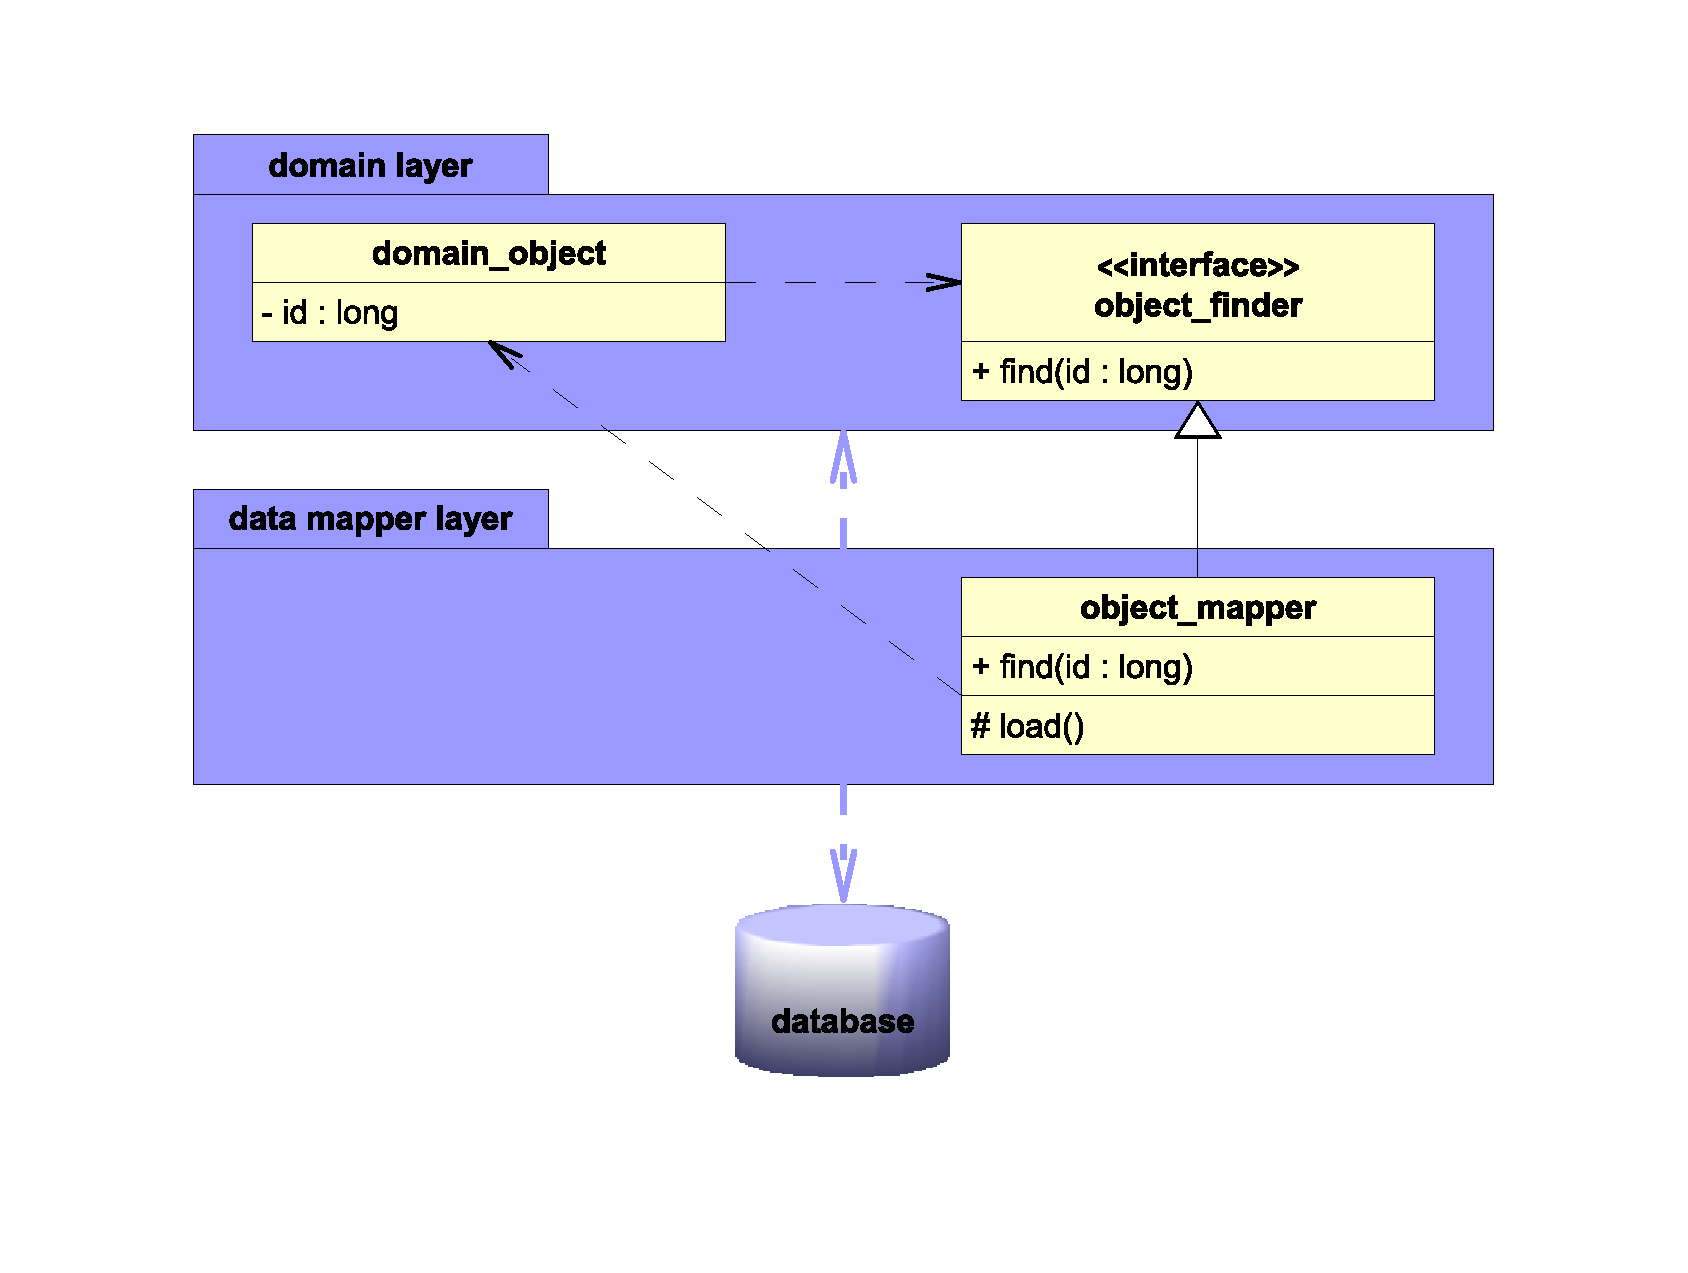
\includegraphics[scale=0.3]{vector/datamapper.eps}
        \caption{Data Mapper Pattern}
        \label{datamapper_figure}
    \end{center}
\end{figure}

The dashed arrows in figure \ref{datamapper_figure} indicate dependencies. The
data mapper layer knows the domain model- as well as the data source layer, via
\emph{unidirectional} relations. Its task is to \emph{translate} between the two,
in both directions. Domain model and data source know nothing from each other.

Each domain model class knows its appropriate interface (\emph{object\_finder})
but does not know the implementation of the same. That is, persistence- and
data retrieval mechanisms are hidden in front of the domain model. The
implementation (\emph{object\_mapper}) is part of the mapping package and also
implements all finder methods. It maps data of the received result sets to the
special attributes of the domain model objects.

The \emph{Mediator} pattern \cite{gamma1995} is similar to the \emph{Mapper}, in
that it is used to decouple different parts of a system. Fowler \cite{fowler2002}
writes: \textit{\ldots the objects that use a mediator are aware of it, even if
they aren't aware of each other; the objects that a mapper separates aren't even
aware of the mapper.}

Although the \emph{Data Mapper} pattern is very helpful at implementing OO
systems, two things are to be criticised:

Firstly, since the \emph{object\_finder} relies on functionality specific to the
retrieval of persistent data, it does actually belong into the data mapper layer
what, if done, would create bidirectional dependencies between the domain model-
and data mapper layer. But also with the \emph{object\_finder} remaining in the
domain model layer, dependencies are not purely unidirectional. It is true that
from an OO view, they are. Internally, however, a super class or interface
relates to its inheriting classes, so that it can call their methods to satisfy
the polymorphic behaviour.

Secondly, the layers do not truely build on each other. Taken a standard
architecture consisting of the following five -- instead of only three -- layers:

\begin{enumerate}
    \item Presentation
    \item Application Process
    \item Domain Model
    \item Data Mapper
    \item Data Source
\end{enumerate}

\ldots the application process does not only access the domain model layer, it
also has to manage (create and destroy) the objects of the data mapper layer.
In other words, it surpasses (disregards) the domain model layer when accessing
the data mapper layer directly.

%
% $RCSfile: data_transfer_object.tex,v $
%
% Copyright (C) 2002-2008. Christian Heller.
%
% Permission is granted to copy, distribute and/or modify this document
% under the terms of the GNU Free Documentation License, Version 1.1 or
% any later version published by the Free Software Foundation; with no
% Invariant Sections, with no Front-Cover Texts and with no Back-Cover
% Texts. A copy of the license is included in the section entitled
% "GNU Free Documentation License".
%
% http://www.cybop.net
% - Cybernetics Oriented Programming -
%
% http://www.resmedicinae.org
% - Information in Medicine -
%
% Version: $Revision: 1.1 $ $Date: 2008-08-19 20:41:06 $ $Author: christian $
% Authors: Christian Heller <christian.heller@tuxtax.de>
%

\subsubsection{Data Transfer Object}
\label{data_transfer_object_heading}
\index{Data Transfer Object Pattern}
\index{DTO}
\index{Assembler Object}
\index{Flat Data Structure}
\index{Translator Architecture}

\begin{figure}[ht]
    \begin{center}
       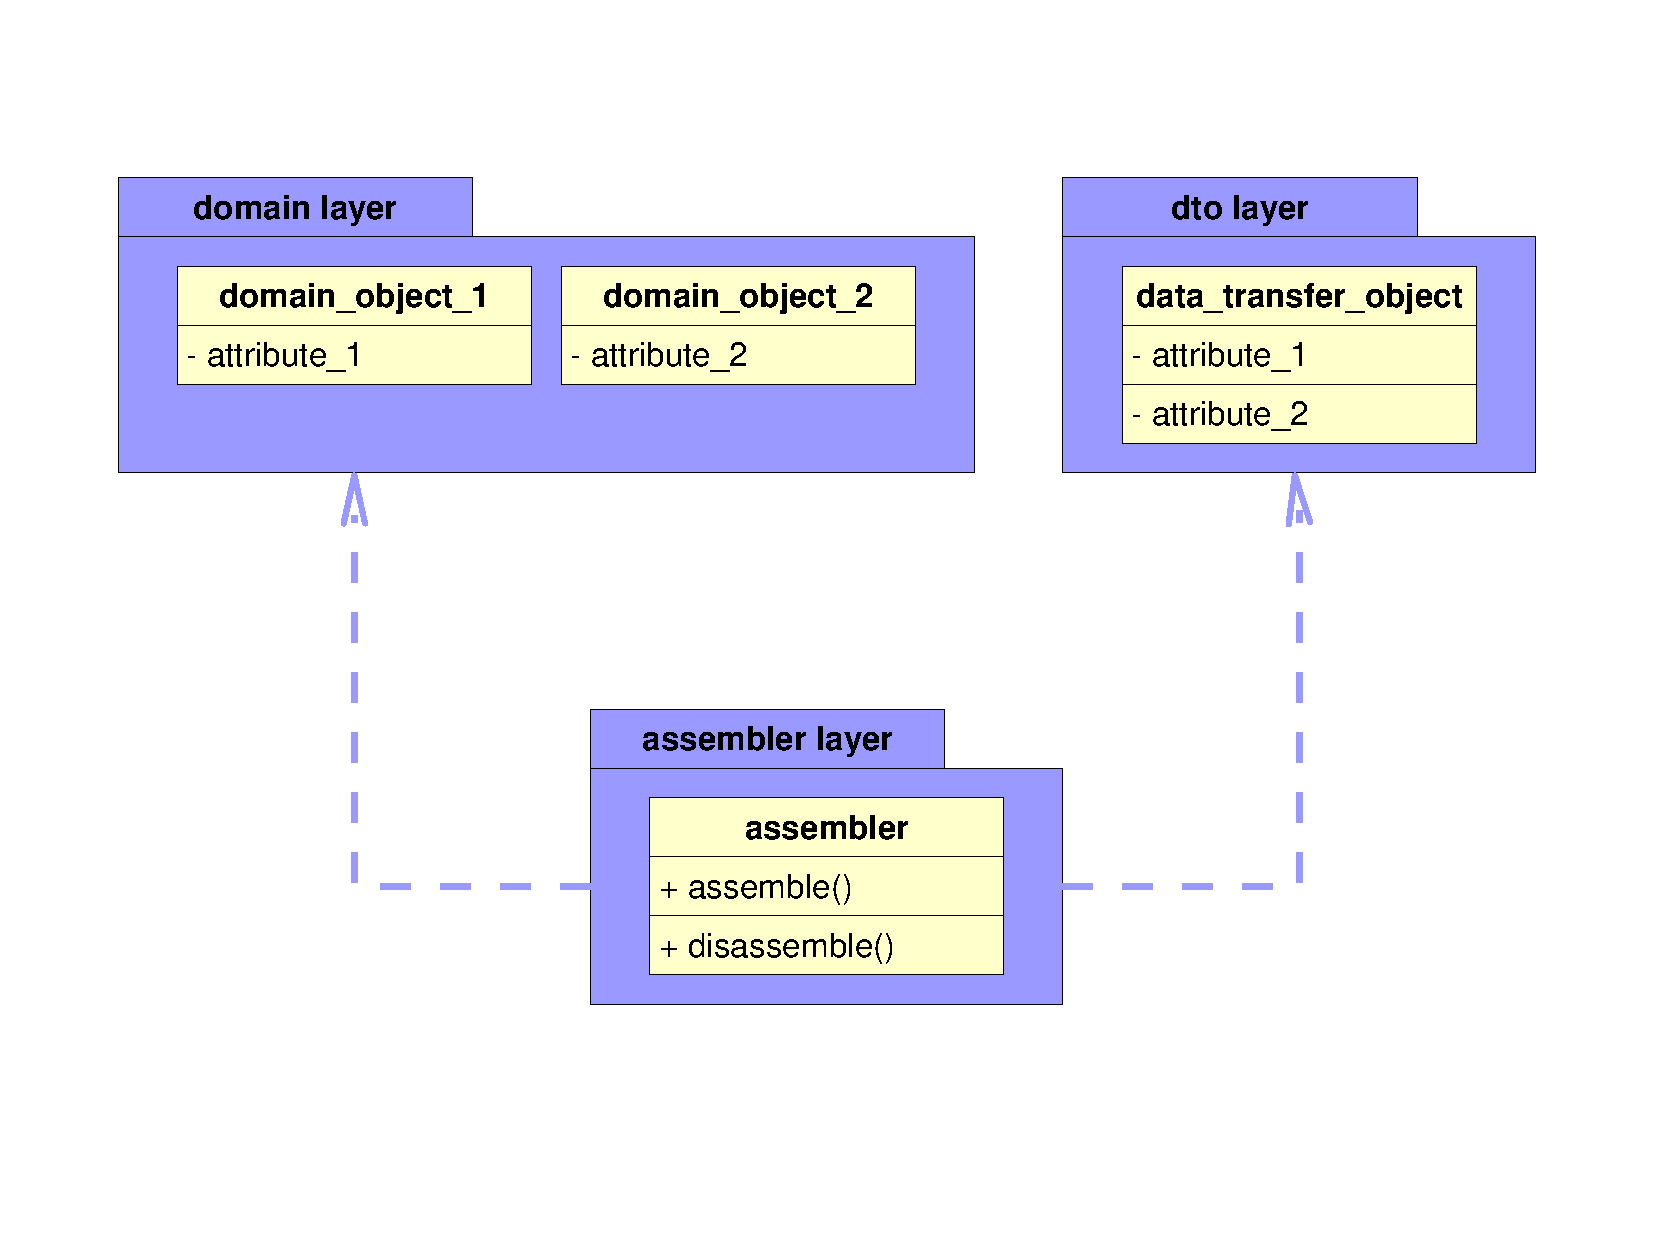
\includegraphics[scale=0.3,angle=-90]{graphic/dto.pdf}
       \caption{Data Transfer Object Pattern}
       \label{dto_figure}
    \end{center}
\end{figure}

It is a well-known fact that many small requests between two processes, and
even more between two hosts in a network need a lot of time. A local machine
with two processes has to permanently change the \emph{Program Context}; a
network has a lot of \emph{Transfers}. For each request, there is a necessity
of at least \emph{two} transfers -- the \emph{Question} of the client and the
\emph{Answer} of the server. Transfer methods are often expected to deliver
common data such as a Person's address, that is surname, first name, street,
zip-code, town and so on. These information is best retrieved by only
\emph{one} transfer call. That way, the client has to wait only once for a
server response and the server does not get too many single tasks. All address
data (in this example) would best be packaged together and sent back to the
client.

A scenario of that kind is exactly what the \emph{Data Transfer Object} pattern
\cite{fowler2002} proposes a solution for: A central \emph{Assembler} object
takes all common data of the server's domain model objects and assembles them
together into a special \emph{Data Transfer Object} (DTO), which is a flat data
structure (figure \ref{dto_figure}). The server will then send this DTO over
network to the client. On the client's side, a similar assembler takes the DTO,
finds out all received data and maps (disassembles) them to the client's domain
model. In that manner, a DTO is able to drastically improve the communication
performance.

Both, \emph{Data Mapper-} and DTO pattern translate one model into another. Due
to this similarity, chapter \ref{state_and_logic_heading} will try to merge
them into a common \emph{Translator} architecture.

%
% $RCSfile: model_view_controller.tex,v $
%
% Copyright (C) 2002-2008. Christian Heller.
%
% Permission is granted to copy, distribute and/or modify this document
% under the terms of the GNU Free Documentation License, Version 1.1 or
% any later version published by the Free Software Foundation; with no
% Invariant Sections, with no Front-Cover Texts and with no Back-Cover
% Texts. A copy of the license is included in the section entitled
% "GNU Free Documentation License".
%
% http://www.cybop.net
% - Cybernetics Oriented Programming -
%
% http://www.resmedicinae.org
% - Information in Medicine -
%
% Version: $Revision: 1.1 $ $Date: 2008-08-19 20:41:07 $ $Author: christian $
% Authors: Christian Heller <christian.heller@tuxtax.de>
%

\subsubsection{Model View Controller}
\label{model_view_controller_heading}
\index{Model View Controller Pattern}
\index{MVC}
\index{Graphical User Interface}
\index{GUI}
\index{Observer Pattern}
\index{Strategy Pattern}
\index{Wrapper Pattern}
\index{Composite Pattern}
\index{Java Foundation Classes}
\index{JFC}
\index{Microsoft Foundation Classes}
\index{MFC}
\index{Document View MVC Variant}
\index{Translator Architecture}

After having had a closer look at design patterns for persistence
(\emph{Data Mapper}) and communication (\emph{Data Transfer Object}), this
section considers the presentation layer of an application (figure
\ref{logical_figure}), which is often realised in form of a
\emph{Graphical User Interface} (GUI). Nowadays, the well-known
\emph{Model View Controller} (MVC) pattern \cite{buschmann, fowler2002} is used
by a majority of standard business applications. Its principle is to have the
\emph{Model} holding domain data, the \emph{View} accessing and displaying
these data and the \emph{Controller} providing the workflow of the application
by handling any action events happening on the view (figure \ref{mvc_figure}).
This separation eases the creation of applications with many synchronous views
on the same data. Internally, the MVC may consist of design patterns like:

\begin{figure}[ht]
    \begin{center}
        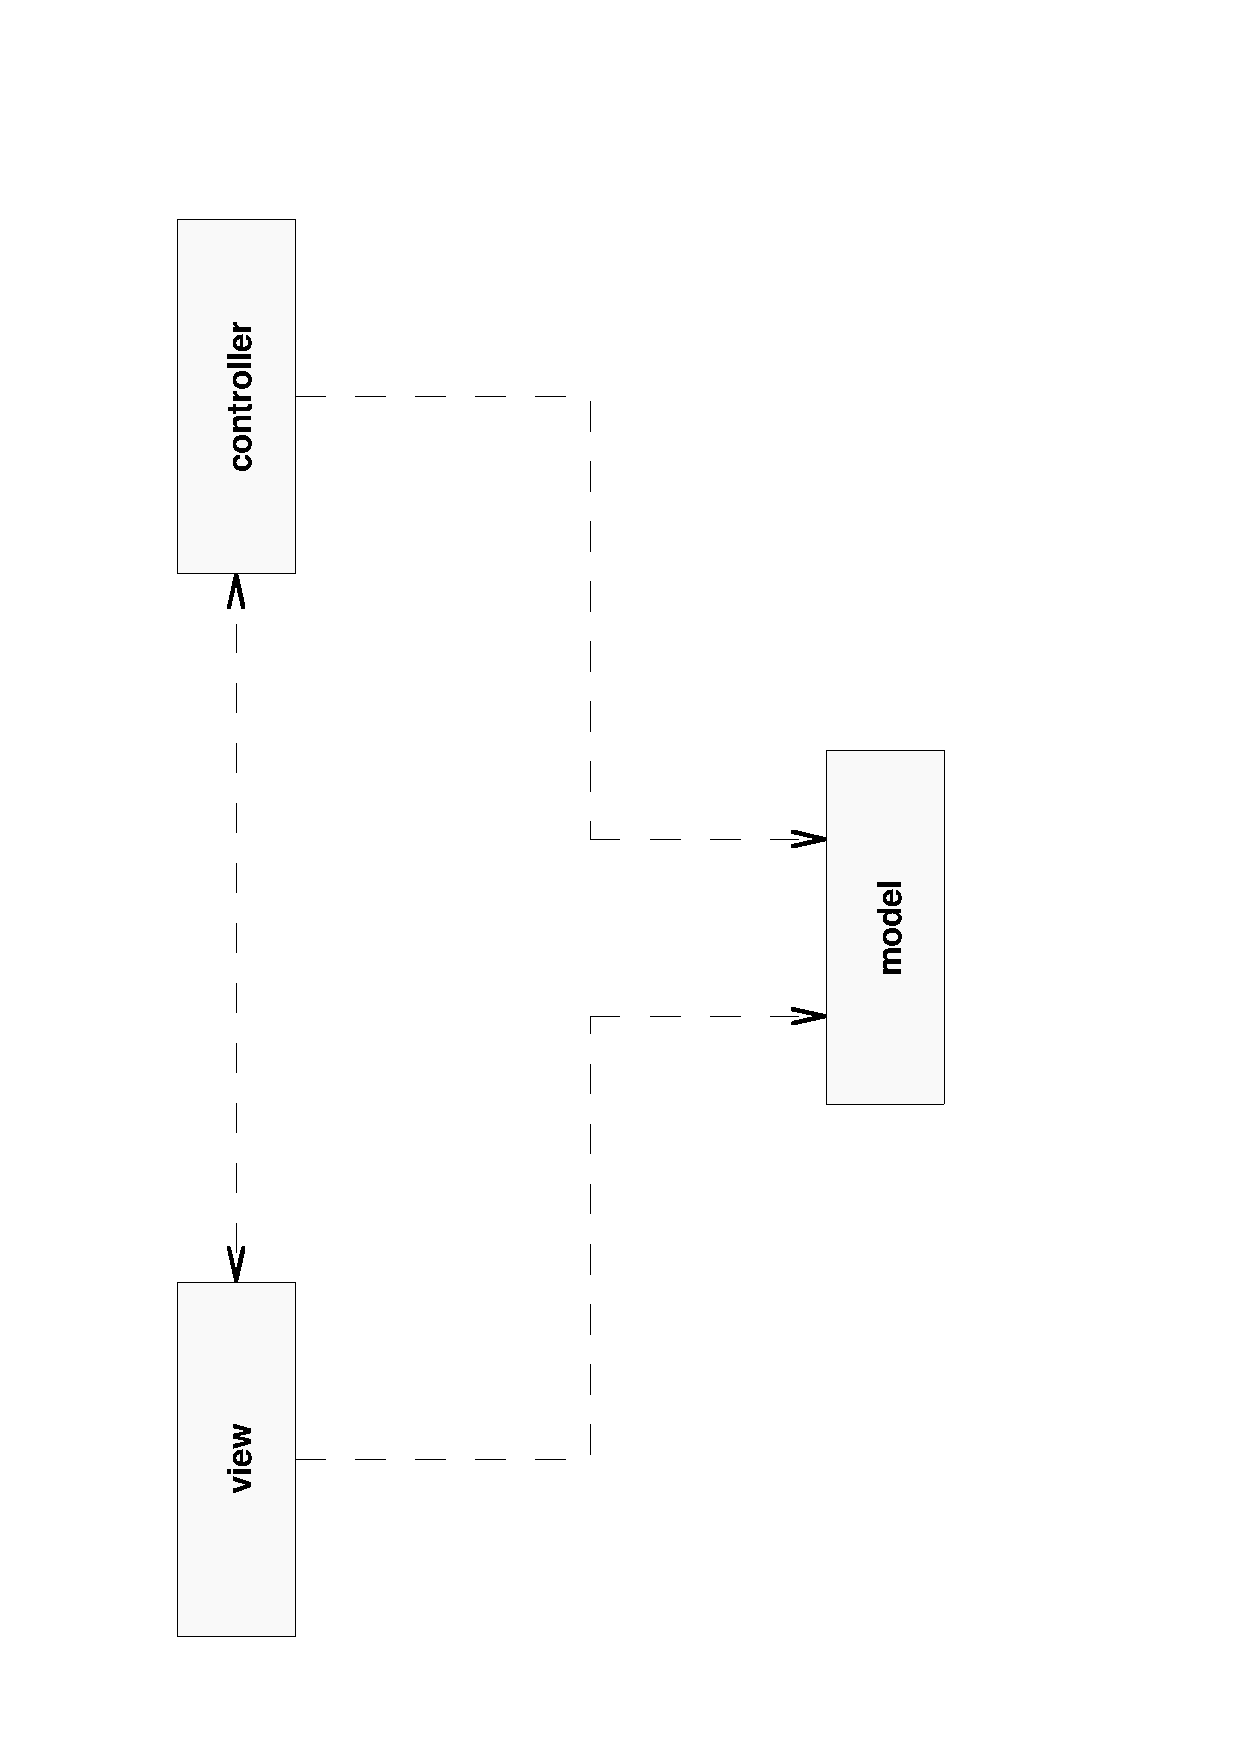
\includegraphics[scale=0.3,angle=-90]{graphic/mvc.pdf}
        \caption{Model View Controller Pattern}
        \label{mvc_figure}
    \end{center}
\end{figure}

\begin{itemize}
    \item[-] \emph{Observer} (section \ref{observer_heading}) which notifies
        the views about data model changes
    \item[-] \emph{Strategy} \cite{gamma1995} which encapsulates exchangeable
        functionality of the controller
    \item[-] \emph{Wrapper} (section \ref{wrapper_heading}) which delegates
        controller functionality to the \emph{Strategy}
    \item[-] \emph{Composite} (section \ref{composite_heading}) which equips
        graphical views with a hierarchical structure
\end{itemize}

Some MVC implementations like parts of the \emph{Java Foundation Classes} (JFC)
use a simplified version not separating controllers from their views. The
\emph{Microsoft Foundation Classes} (MFC) C++ library calls its implementation
\emph{Document-View}.

Besides the above-mentioned patterns \emph{Data Mapper} and DTO, MVC is the
third one getting merged into a common \emph{Translator} architecture, in
chapter \ref{state_and_logic_heading}.

%
% $RCSfile: hierarchical_model_view_controller.tex,v $
%
% Copyright (C) 2002-2008. Christian Heller.
%
% Permission is granted to copy, distribute and/or modify this document
% under the terms of the GNU Free Documentation License, Version 1.1 or
% any later version published by the Free Software Foundation; with no
% Invariant Sections, with no Front-Cover Texts and with no Back-Cover
% Texts. A copy of the license is included in the section entitled
% "GNU Free Documentation License".
%
% http://www.cybop.net
% - Cybernetics Oriented Programming -
%
% http://www.resmedicinae.org
% - Information in Medicine -
%
% Version: $Revision: 1.1 $ $Date: 2008-08-19 20:41:07 $ $Author: christian $
% Authors: Christian Heller <christian.heller@tuxtax.de>
%

\subsubsection{Hierarchical Model View Controller}
\label{hierarchical_model_view_controller_heading}
\index{Hierarchical Model View Controller Pattern}
\index{HMVC}
\index{Model View Controller Pattern}
\index{MVC}
\index{Composite Pattern}
\index{Layers Pattern}
\index{Chain of Responsibility Pattern}
\index{Presentation Layer}
\index{MVC Triad}
\index{Presentation Abstraction Control}
\index{PAC}
\index{PAC Agent}

There exist several extensions of the MVC pattern, one of them being the
\emph{Hierarchical Model View Controller} (HMVC) \cite{cai}. It combines the
patterns \emph{Composite} (section \ref{composite_heading}), \emph{Layers}
(section \ref{layers_heading}) and \emph{Chain of Responsibility} (section
\ref{chain_of_responsibility_heading}) into one conceptual architecture (figure
\ref{hmvc_figure}). This architecture divides the presentation layer into
hierarchical sections containing so-called \emph{MVC Triads}. The triads
conventionally consist of \emph{Model}, \emph{View} and \emph{Controller},
each. They communicate with each other by relating over their controller
object. Following the \emph{Layers} pattern, only neighbouring layers know from
each other.

\begin{figure}[ht]
    \begin{center}
        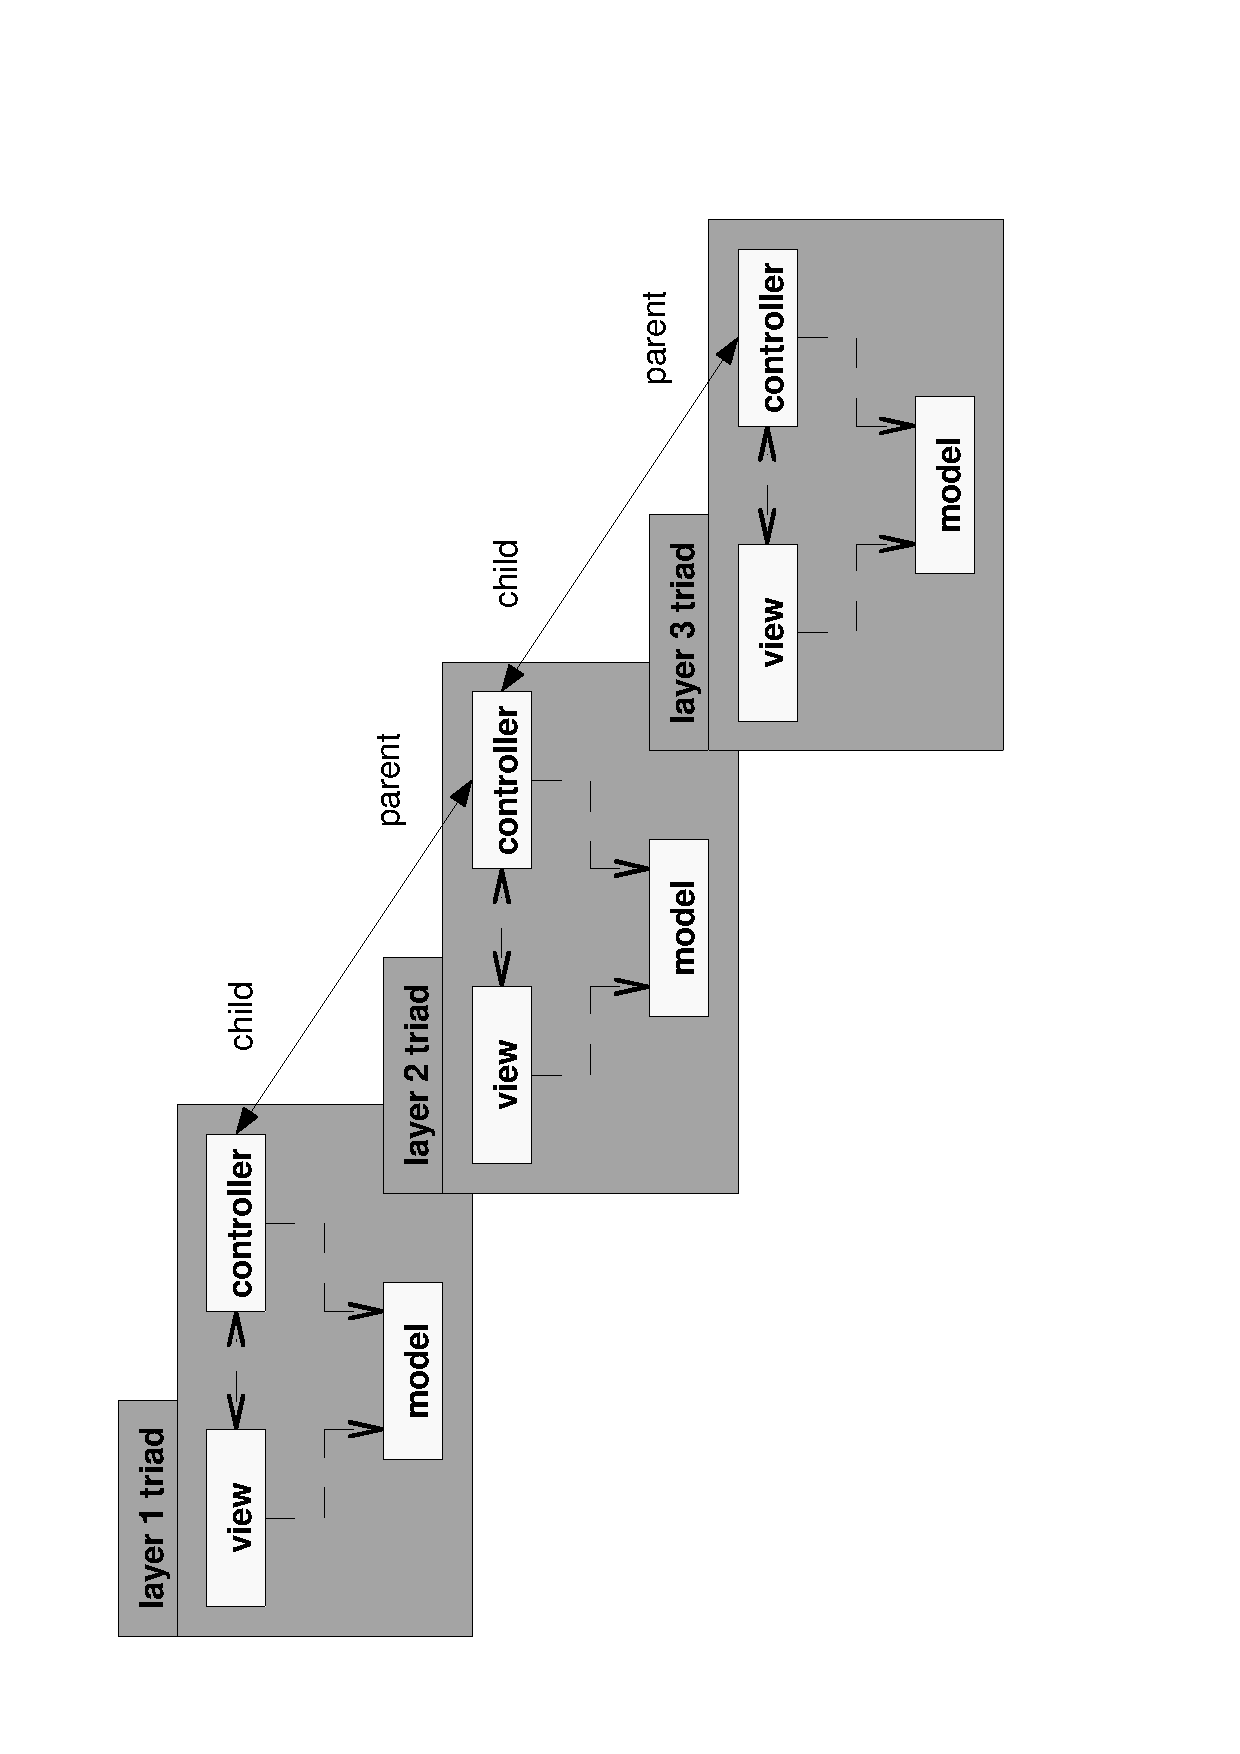
\includegraphics[scale=0.3,angle=-90]{graphic/hmvc.pdf}
        \caption{Hierarchical Model View Controller Pattern}
        \label{hmvc_figure}
    \end{center}
\end{figure}

As a practical example, the upper-most triad could represent a graphical
\emph{Dialogue} and the next lower one a \emph{Panel}. Being a container, too,
the panel could hold a third triad like for example a \emph{Button}. Events
occuring at the button are then normally processed by the corresponding
controller belonging to the button's triad. If, however, the button controller
cannot handle the event, that is forwarded along the chain of responsibility to
the controller of the higher-next layer. If also the panel controller does not
know how to handle the event, the final responsibility falls to the controller
of the dialogue's triad.

The HMVC is similar to the \emph{Presentation Abstraction Control} (PAC) pattern
\cite{buschmann}. A \emph{PAC Agent} is comparable to an \emph{HMVC Triad}.

Chapter \ref{knowledge_schema_heading} will apply the principle of
\emph{Hierarchy} not only to logic- (controller), but also to user interface-
(view), domain- and further models.

%
% $RCSfile: microkernel.tex,v $
%
% Copyright (c) 2004. Christian Heller. All rights reserved.
%
% No copying, altering, distribution or any other actions concerning this
% document, except after explicit permission by the author!
% At some later point in time, this document is planned to be put under
% the GNU FDL license. For now, _everything_ is _restricted_ by the author.
%
% http://www.cybop.net
% - Cybernetics Oriented Programming -
%
% http://www.resmedicinae.org
% - Information in Medicine -
%
% @author Christian Heller <christian.heller@tuxtax.de>
%

\paragraph{Microkernel}
\label{microkernel_heading}

The \emph{Microkernel} pattern \cite{buschmann} allows to keep a system flexible
and adaptable to changing requirements or new technologies. A minimal functional
\emph{Kernel} gets separated from extended functionality. The kernel may call
internal- or external servers (figure \ref{microkernel_figure}) to let them
solve special tasks which do not belong to its own core responsibility. Internal
servers are often called \emph{Daemons}.

\begin{figure}[ht]
    \begin{center}
        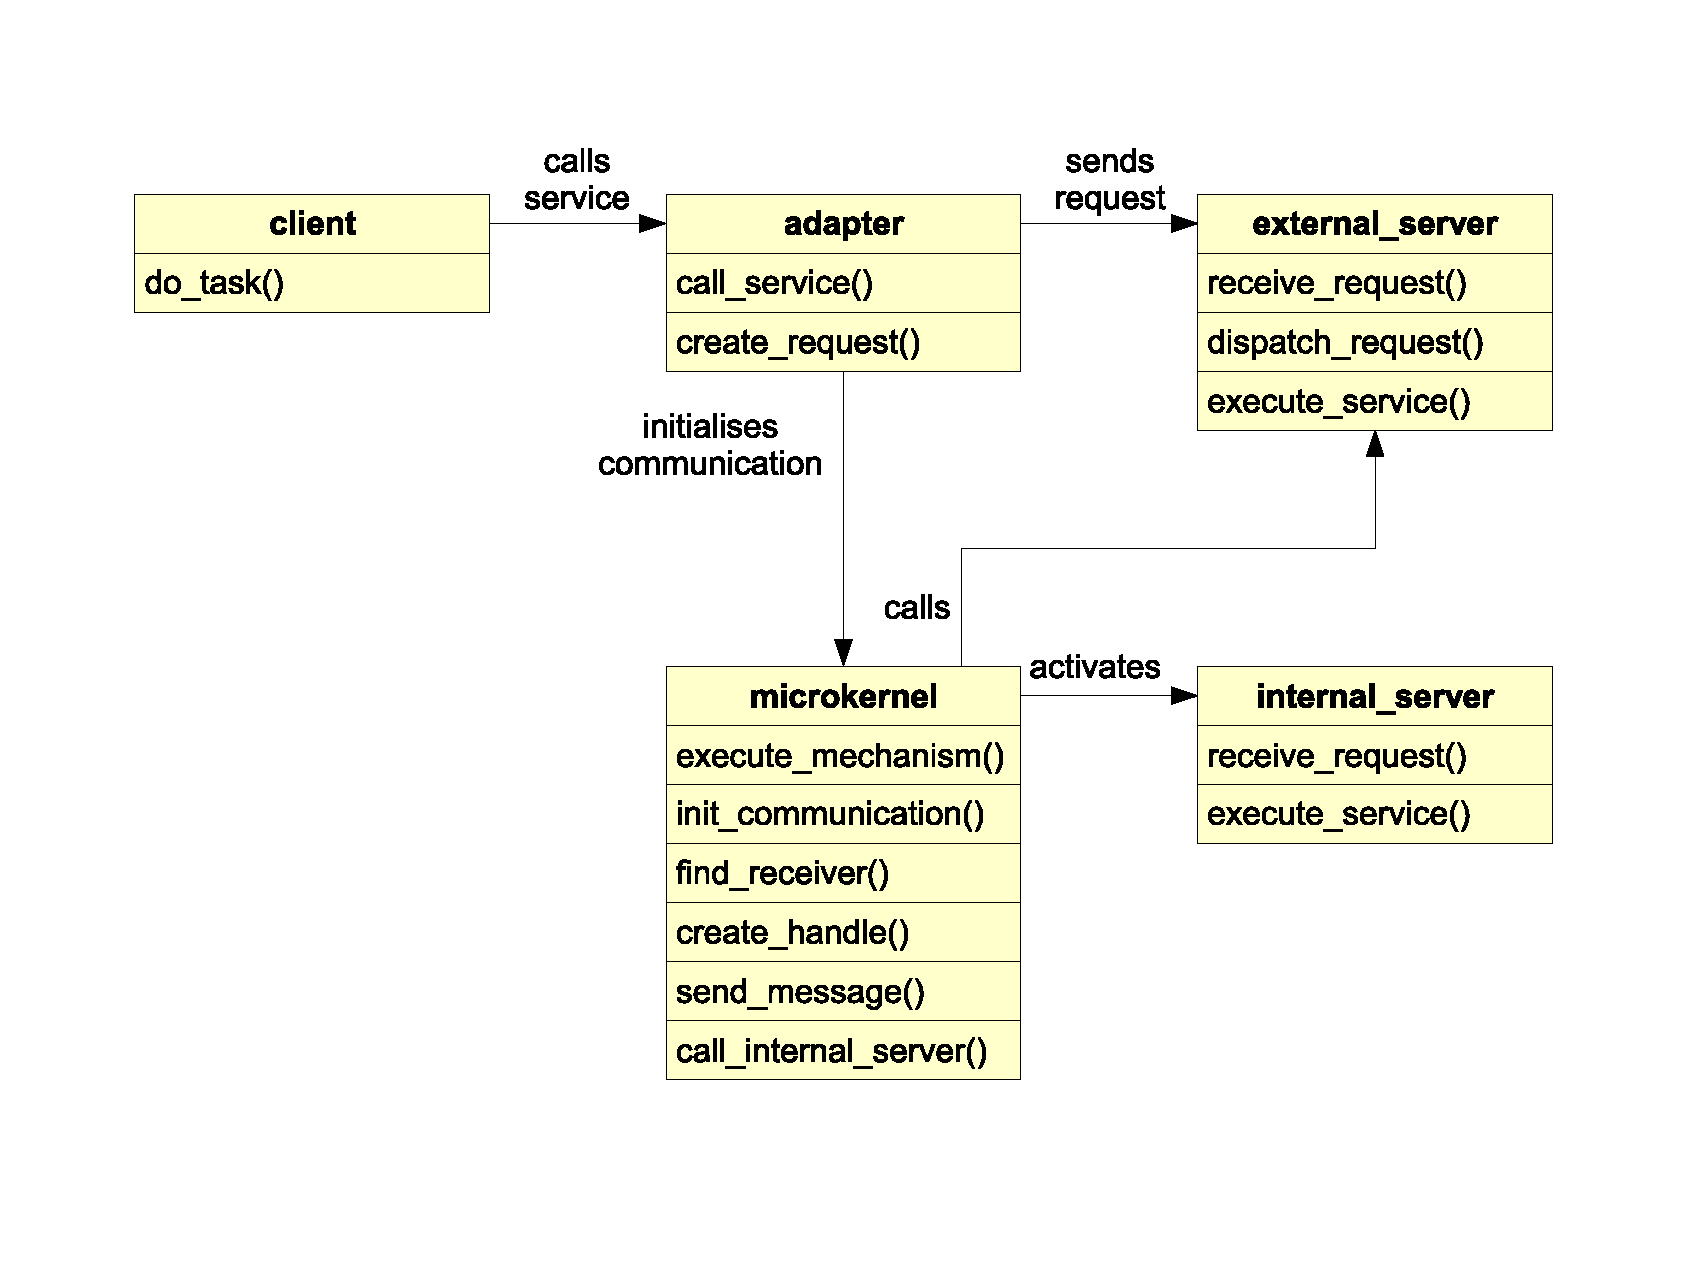
\includegraphics[scale=0.3]{vector/microkernel.eps}
        \caption{Microkernel Pattern}
        \label{microkernel_figure}
    \end{center}
\end{figure}

This pattern provides a \emph{Plug \& Play} environment and serves as base
architecture for many modern \emph{Operating Systems} (OS). Andrew S. Tanenbaum
recommends its use as well \cite{tanenbaum2001}.

%
% $RCSfile: broker.tex,v $
%
% Copyright (C) 2002-2008. Christian Heller.
%
% Permission is granted to copy, distribute and/or modify this document
% under the terms of the GNU Free Documentation License, Version 1.1 or
% any later version published by the Free Software Foundation; with no
% Invariant Sections, with no Front-Cover Texts and with no Back-Cover
% Texts. A copy of the license is included in the section entitled
% "GNU Free Documentation License".
%
% http://www.cybop.net
% - Cybernetics Oriented Programming -
%
% http://www.resmedicinae.org
% - Information in Medicine -
%
% Version: $Revision: 1.1 $ $Date: 2008-08-19 20:41:05 $ $Author: christian $
% Authors: Christian Heller <christian.heller@tuxtax.de>
%

\subsubsection{Broker}
\label{broker_heading}
\index{Broker Pattern}
\index{Distributed Application}

The \emph{Broker} pattern \cite{buschmann} may support the creation of an IT
infrastructure for distributed applications. It connects decoupled components
which interact through remote service invocations (figure \ref{broker_figure}).
The broker is responsible for coordinating all communication, for forwarding
requests as well as for transmitting results and exceptions.

%
% CAUTION! This file actually contains a graphics, which was moved to
% the 'microkernel.tex' file, for better formatting results in the document.
%

Chapter \ref{cybernetics_oriented_interpreter_heading} introduces an
interpreter program being able to act as broker.

%
% $RCSfile: pipes_and_filters.tex,v $
%
% Copyright (C) 2002-2008. Christian Heller.
%
% Permission is granted to copy, distribute and/or modify this document
% under the terms of the GNU Free Documentation License, Version 1.1 or
% any later version published by the Free Software Foundation; with no
% Invariant Sections, with no Front-Cover Texts and with no Back-Cover
% Texts. A copy of the license is included in the section entitled
% "GNU Free Documentation License".
%
% http://www.cybop.net
% - Cybernetics Oriented Programming -
%
% http://www.resmedicinae.org
% - Information in Medicine -
%
% Version: $Revision: 1.1 $ $Date: 2008-08-19 20:41:08 $ $Author: christian $
% Authors: Christian Heller <christian.heller@tuxtax.de>
%

\subsubsection{Pipes and Filters}
\label{pipes_and_filters_heading}
\index{Pipes and Filters Pattern}
\index{Push Scenario for Data Forwarding}
\index{Pull Scenario for Data Forwarding}
\index{Mixed Push-Pull-Pipeline Scenario for Data Forwarding}
\index{Independent Loops Scenario for Data Forwarding}

Systems that process streams of data may make use of the \emph{Pipes and Filters}
pattern \cite{buschmann}. It encapsulates every processing step in an own
\emph{Filter} component and forwards the data through channels which are called
\emph{Pipeline} (figure \ref{pipesfilters_figure}). The data forwarding can
follow various scenarios:

\begin{figure}[ht]
    \begin{center}
        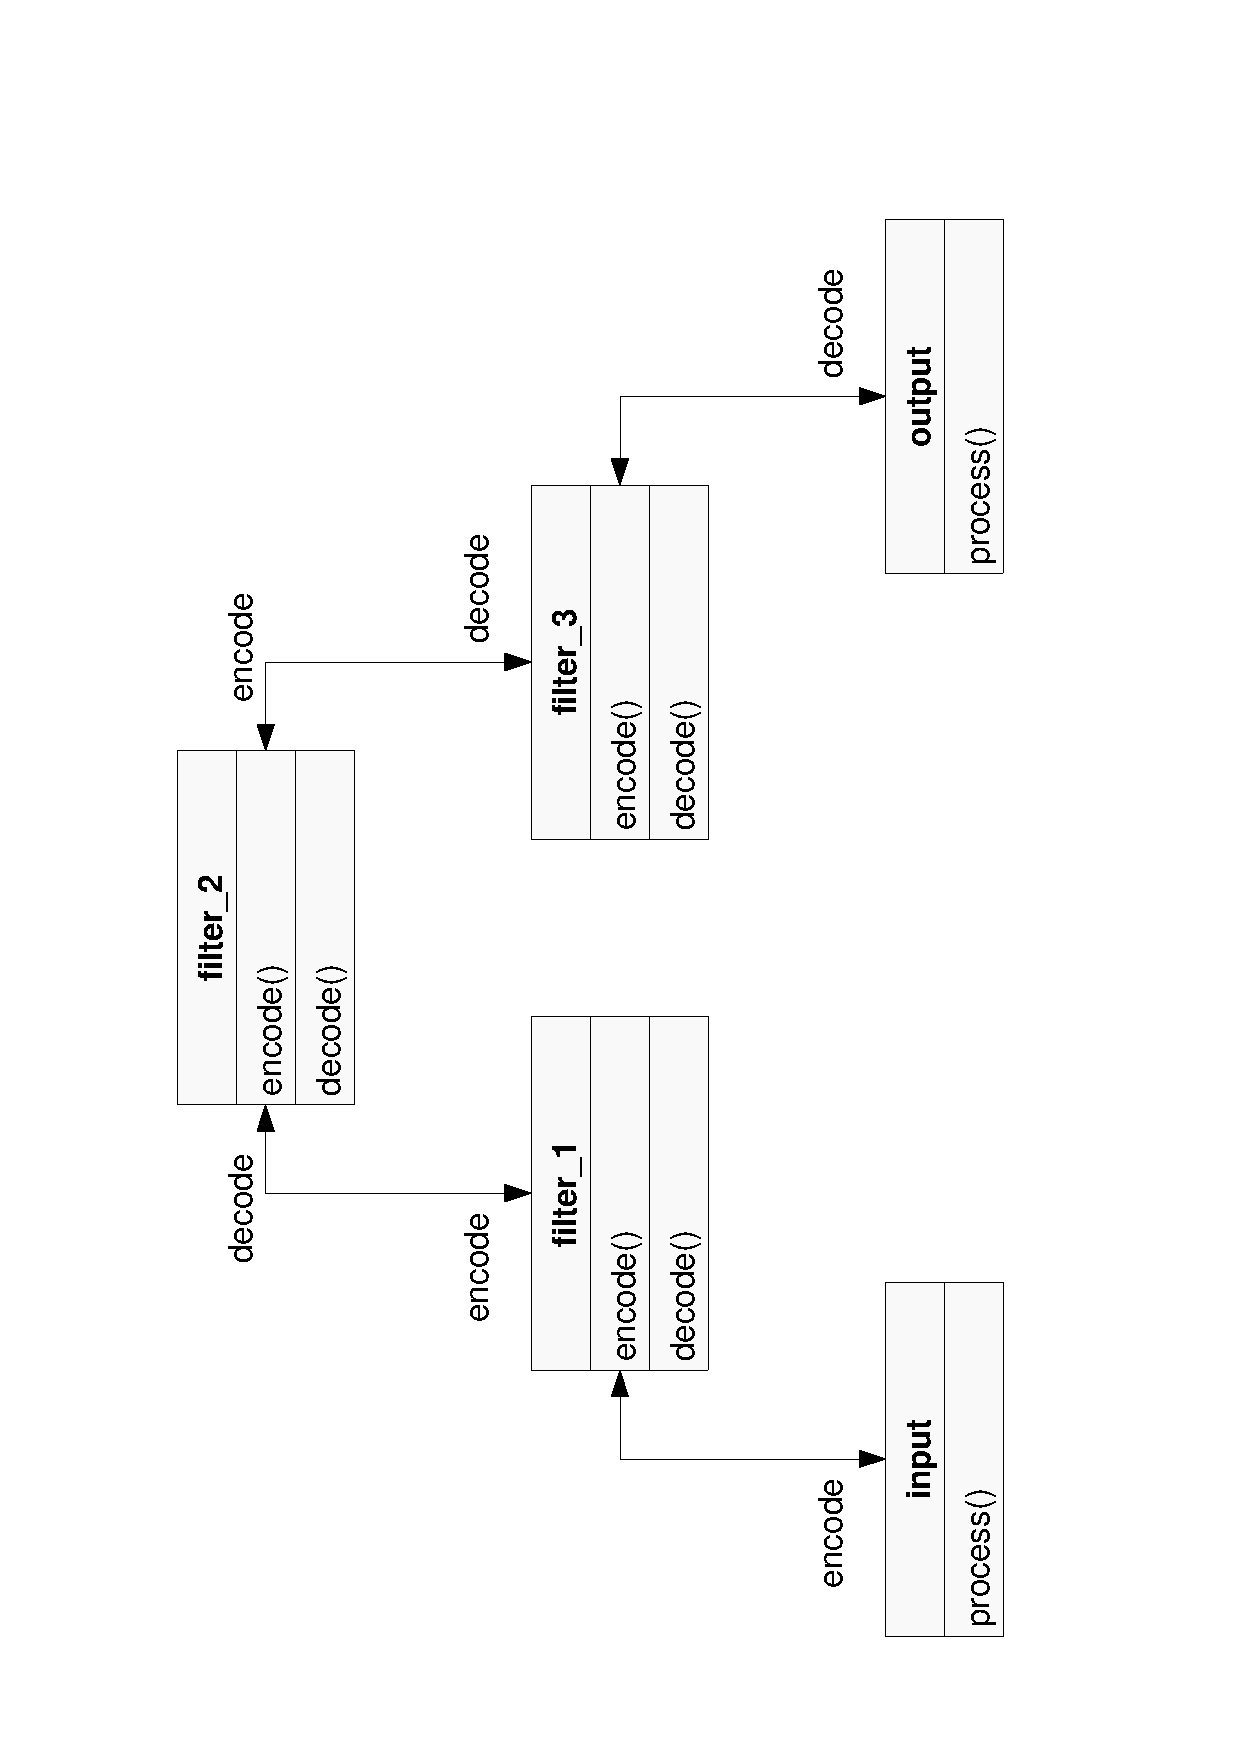
\includegraphics[scale=0.3,angle=-90]{graphic/pipesfilters.pdf}
        \caption{Pipes and Filters Pattern}
        \label{pipesfilters_figure}
    \end{center}
\end{figure}

\begin{itemize}
    \item[-] \emph{Push:} active filter pushes data to passive filter
    \item[-] \emph{Pull:} active filter pulls data from passive filter
    \item[-] \emph{Mixed Push-Pull-Pipeline:} all filters may push or pull data
    \item[-] \emph{Independent Loops:} all filters are active and access pipeline data
\end{itemize}

Families of related systems can be formed by changing the single filter
positions. Special communication filters are also used in the interpreter
program of chapter \ref{cybernetics_oriented_interpreter_heading}. Its filters
belong to neither of the above-listed forms of data forwarding, because they
are all passive, controlled from an outside entity which is not a filter
itself.

%
% $RCSfile: reflection.tex,v $
%
% Copyright (c) 2004. Christian Heller. All rights reserved.
%
% No copying, altering, distribution or any other actions concerning this
% document, except after explicit permission by the author!
% At some later point in time, this document is planned to be put under
% the GNU FDL license. For now, _everything_ is _restricted_ by the author.
%
% http://www.cybop.net
% - Cybernetics Oriented Programming -
%
% http://www.resmedicinae.org
% - Information in Medicine -
%
% @author Christian Heller <christian.heller@tuxtax.de>
%

\paragraph{Reflection}
\label{reflection_heading}

The \emph{Reflection} pattern \cite{buschmann} (also known under the synonyms
\emph{Open Implementation} or \emph{Meta-Level Architecture}) provides a
mechanism to change the structure and behaviour of a software system
\emph{dynamically}, that is at runtime, which is why that mechanism is sometimes
called \emph{Run Time Type Identification} (RTTI). A reflective system owns
information about itself and uses these to remain changeable and extensible.

\begin{figure}[ht]
    \begin{center}
        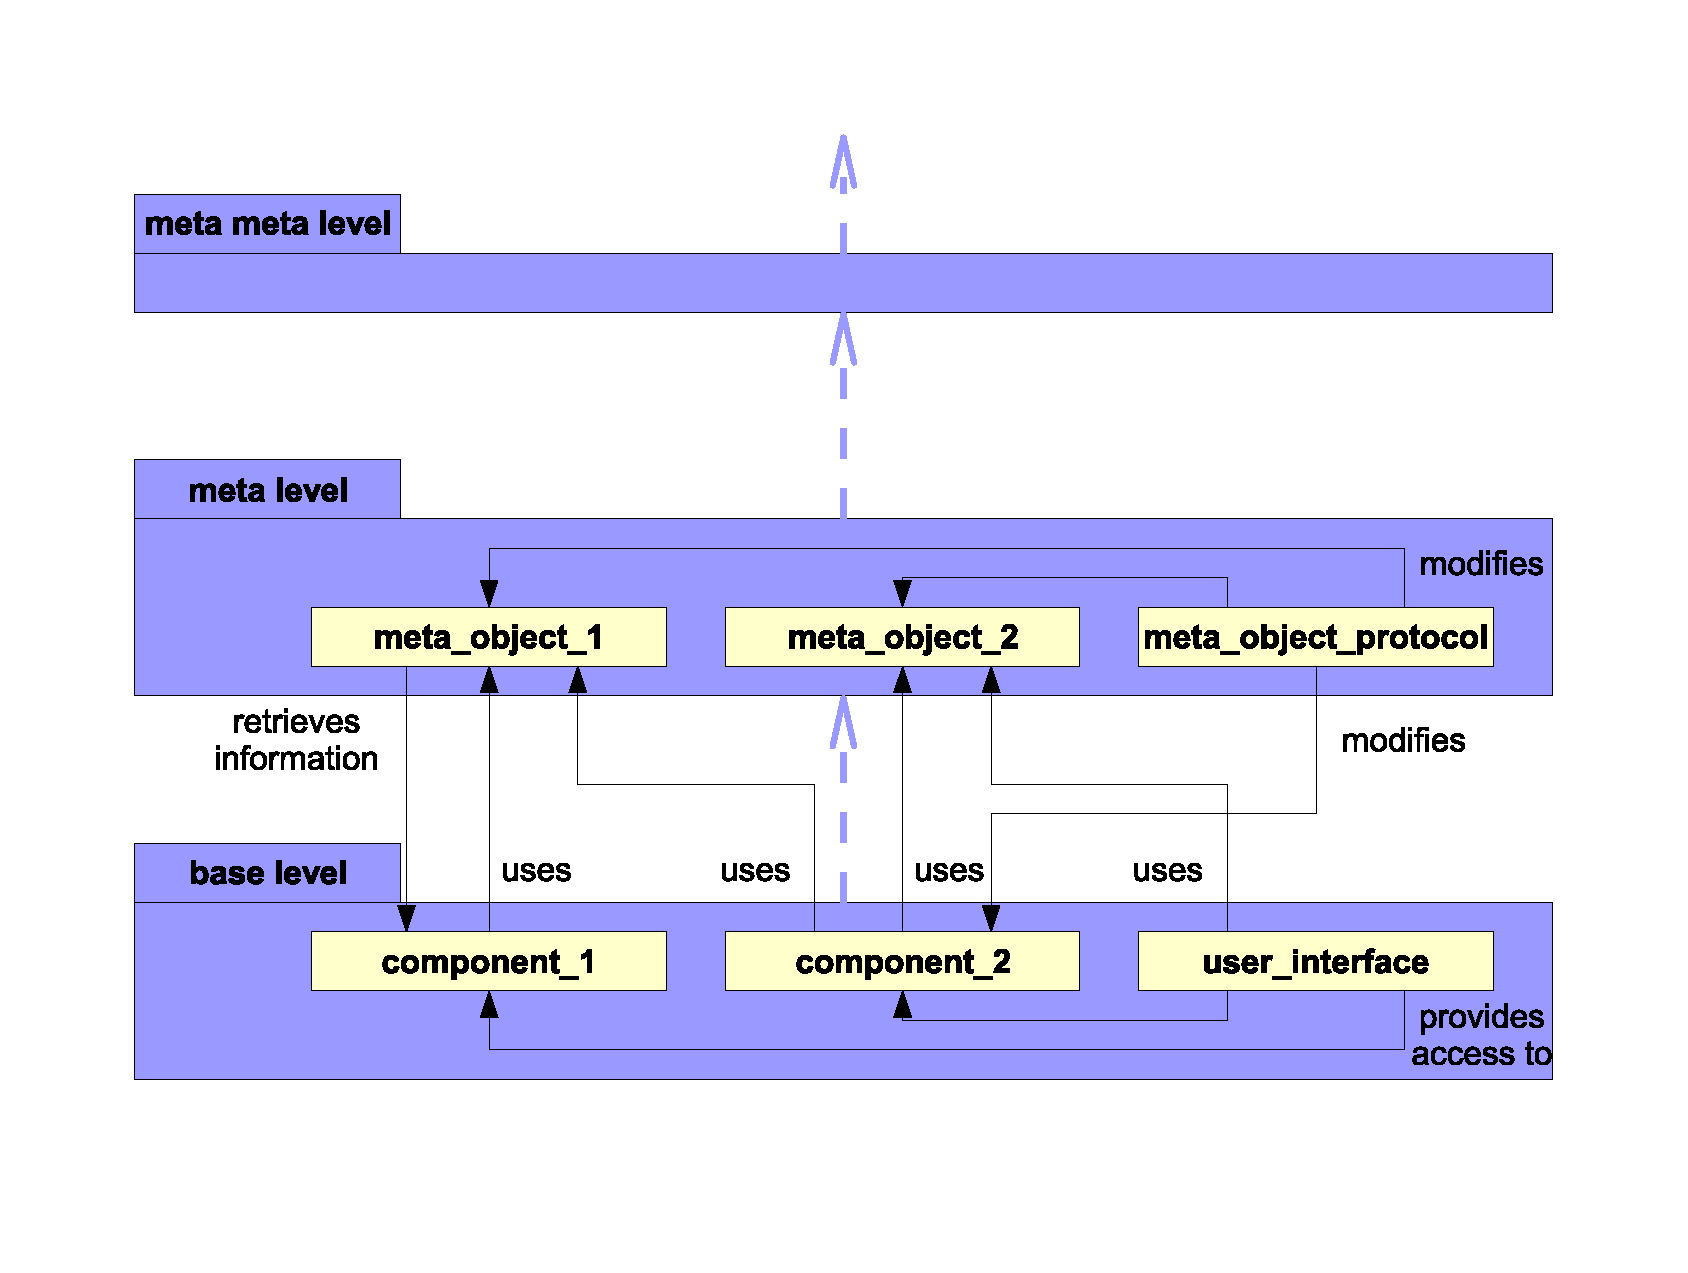
\includegraphics[scale=0.3]{vector/reflection.eps}
        \caption{Reflection Pattern}
        \label{reflection_figure}
    \end{center}
\end{figure}

Reflective information \emph{about} something is called \emph{Meta Information}.
Therefore, the level above the \emph{Base Level} in figure \ref{reflection_figure}
is labelled \emph{Meta Level}. The base level depends on the meta level, so that
changes in the meta level will also affect the base level. All manipulation of
meta objects happens through an interface called \emph{Meta Object Protocol}
(MOP), which is responsible for checking the correctness of- and for performing
a change. If a further level holds information about the meta level, then that
additional level is called \emph{Meta Meta Level}, and so forth.

Many examples of meta level architectures exist. In his book
\emph{Analysis Patterns} \cite{fowler1997}, Fowler uses them extensively.
He talks of \emph{Knowledge Level} (instead of meta level) and
\emph{Operational Level} (instead of base level). Elements of the
\emph{Unified Modeling Language} (UML) are defined in an own meta model
\cite{uml}. And the principles of reflection are also supported by several
programming languages, such as \emph{Smalltalk} \cite{smalltalk} and
\emph{Java} \cite{java}.

Classes (types) in a system have a static structure, as defined by the developer
at design time. Normally, most classes belong to the base level containing the
application logic. As written before, one way to change the structure and
behaviour of classes at runtime is to introduce a meta level providing type
information, in other words functionality that \emph{all} application classes
need. This helps avoid redundant implementations of the same functionality.

Looking closer at functionality, it turns out that some basic features like
persistence and communication occur repeatedly in almost all systems, while
other parts are specific to one concrete application. Traditionally, the
application classes in the base level have to cope with general system
functionality although that is not in their original interest. It therefore
seems logical to try to divide application- and system functionality, and to put
the latter into a meta level.

%
% $RCSfile: broken_type_system.tex,v $
%
% Copyright (c) 2004. Christian Heller. All rights reserved.
%
% No copying, altering, distribution or any other actions concerning this
% document, except after explicit permission by the author!
% At some later point in time, this document is planned to be put under
% the GNU FDL license. For now, _everything_ is _restricted_ by the author.
%
% http://www.cybop.net
% - Cybernetics Oriented Programming -
%
% http://www.resmedicinae.org
% - Information in Medicine -
%
% @author Christian Heller <christian.heller@tuxtax.de>
%

\subsection{Broken Type System}
\label{broken_type_system_heading}

Languages like \emph{Smalltalk} or the \emph{Common Lisp Object System} (CLOS)
offer reflective mechanisms \cite{buschmann}. The \emph{C++ Standard Library},
also known as \emph{libstdc++} \cite{libstdcpp}, has a \emph{type\_info} class
providing meta information that \emph{C++} innately does not have.

In the \emph{Java} framework \cite{java}, finally, the basic \emph{java.lang.*}
package contains the top-most super class \emph{java.lang.Object}. All other
classes in the framework inherit from it. Additionally, the package contains a
class \emph{java.lang.Class} which, among others, keeps reflective (meta) type
information about a \emph{Java} class':

\begin{itemize}
    \item[-] Package
    \item[-] Name
    \item[-] Superior Class
    \item[-] Interfaces
    \item[-] Fields
    \item[-] Methods
    \item[-] Constructors
    \item[-] Modifiers
    \item[-] Member Classes
\end{itemize}

\begin{figure}[ht]
    \begin{center}
        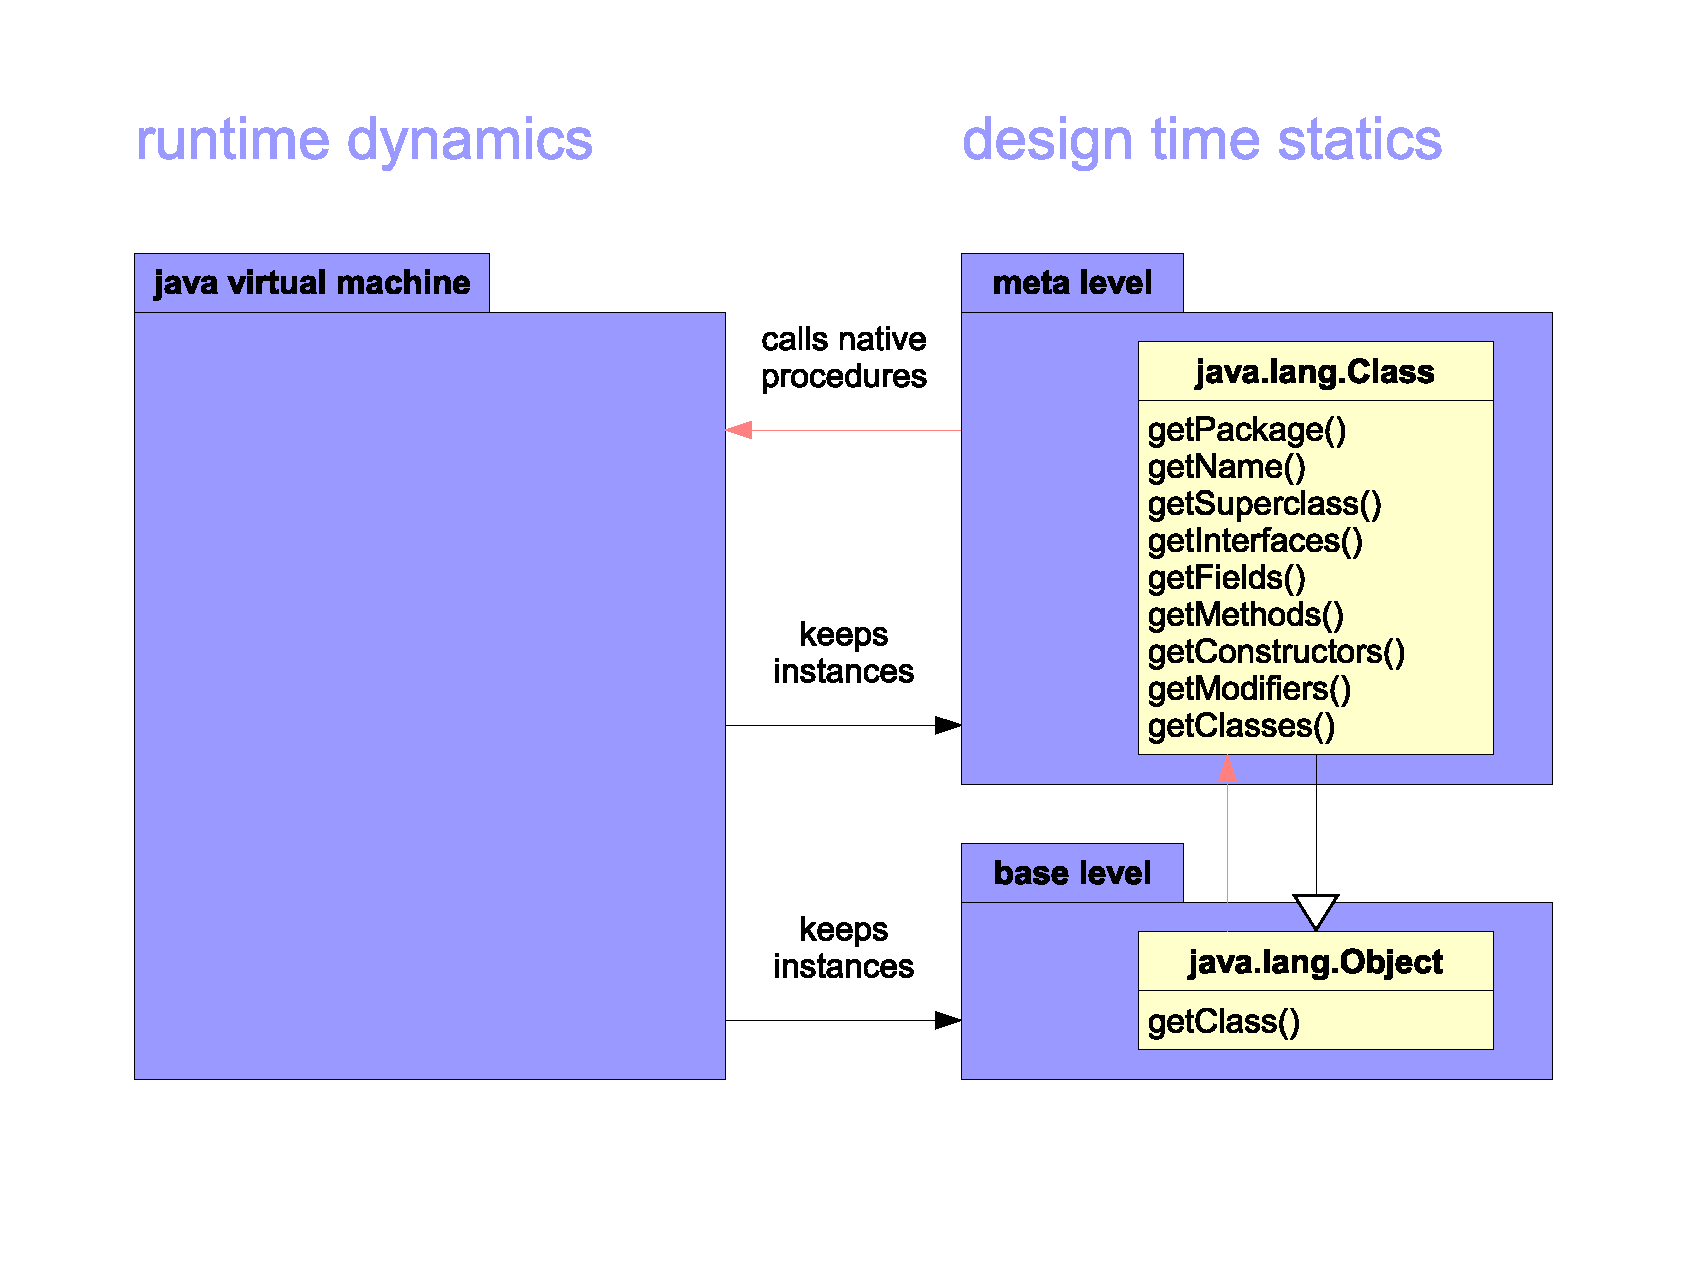
\includegraphics[scale=0.3]{vector/typesystem.eps}
        \caption{Java Type System}
        \label{typesystem_figure}
    \end{center}
\end{figure}

Via the \emph{getClass()} method which they inherit from \emph{java. lang.Object}
(figure \ref{typesystem_figure}), all Java classes have access to that reflective
information in their meta class. The meta class \emph{java.lang.Class} itself
uses so-called \emph{native} methods to access the information in the
\emph{Java Virtual Machine} (JVM).

The JVM operates on a level underneath the actual application, close to the
\emph{Operating System} (OS). It interprets the Java application source code and
resolves all object-oriented- into procedural structures, and finally low-level
system instructions. All runtime objects, that is class instances, are hold in
dynamic structures internal to the JVM. That is why \emph{native} methods need
to be used to access and change the runtime structure or behaviour of objects.

One problem that becomes obvious when inspecting figure \ref{typesystem_figure}
is the existence of a \emph{Bidirectional Dependency}, also called
\emph{Circular Reference}. The two sub dependencies causing it are:

\begin{enumerate}
    \item \emph{Inheritance} of \emph{java.lang.Class} from \emph{java.lang.Object}
        which is due to the rule that all Java classes need to inherit from the
        top-most framework class
    \item \emph{Association} from \emph{java.lang.Object} to \emph{java.lang.Class}
        which enables every object to access its meta class using the
        \emph{getClass()} method
\end{enumerate}

The avoidance of circular references is one of the most basic principles of
computer programming (section \ref{bidirectional_dependency_heading}). The
disadvantage of bidirectional dependencies between meta- and basic level is
also mentioned by Buschmann \cite{buschmann}. If meta classes in the kind of
\emph{java.lang.Class} define the structure and behaviour of all basic classes
inheriting from \emph{java.lang. Object}, then those meta classes in turn should
\emph{not} themselves inherit from \emph{java.lang.Object}.

Another problem is the mixed and redundant storage of meta information which
Jonathon Tidswell \cite{josgeneral} even calls a \emph{Broken Type System}. He
writes: \textit{A careful examination of the classes in the standard runtime will
show that they are not strictly instances of java.lang.Class (hint: statics).}
Gilbert Carl Herschberger II \cite{josgeneral} calls the separation of
reflection and wrappers an \emph{Inconsistent Design}. Java classes are based
on many different kinds of type information:

\begin{itemize}
    \item[-] Structure applied by the JVM through the usage of the \emph{class} keyword
    \item[-] Meta information supplied by the \emph{java.lang.Class} class
    \item[-] Reflective information provided by \emph{java.lang.reflect.*}
    \item[-] Wrapper classes for primitive types in \emph{java.lang.*}
    \item[-] Dynamically created array classes, without having an array class file
\end{itemize}

The fact that the \emph{java.lang.Class} class which is to provide meta
information \emph{about} classes is a \emph{Class} itself is an antagonism. It
is true that that meta class is made \emph{final} to avoid its extension by
inheriting subclasses. But correctly, it should not be a class at all.

Yet how can this paradoxon be resolved? Obviously, one of the two dependencies
between \emph{java.lang.Object} and \emph{java.lang.Class} needs to be cut. But
then either the \emph{java.lang. Object} class would not be able to access its meta
information anymore or the \emph{java.lang.Class} class would not be available as
runtime object to other polymorphic data structures. One solution could be to
merge both classes, so that each object, by default, has the necessary methods
to access its meta information. But as it turns out, this would not be a real
solution, just a \emph{Shift} of the problem to another level. As mentioned above,
the JVM keeps all instances (objects) in internal, dynamic structures. If objects
were allowed to access these internal structures via native methods (procedures),
a similar kind of bidirectional dependency, between the JVM and its stored objects,
would occur.

One finally has to ask whether the usage and manipulation of meta information is
really necessary at all! If objects did not have a \emph{static} structure
consisting of certain attributes and methods, as defined by the software
developer at design time, but instead based on a uniform, \emph{dynamically}
changeable structure -- the need to use reflective mechanisms might disappear.
More research has to be done on this topic.

There are other Java-related points to be criticised. Although it is worth
noting they exist, these are \emph{not} explained in detail here, since this
document wants to focus on general concepts. Gilbert Carl Herschberger II
\cite{josgeneral} mentions the problematic issue of \emph{Pre-Conditions},
leading to corresponding \emph{Assumptions}. After him, such work-arounds were
necessary to break circular references in Java:

\begin{itemize}
    \item[-] Each JVM must pre-define an \emph{Internal Meta Class}, implemented
        in machine code and \emph{not} available as Java bytecode in a class file.
        The \emph{java.lang.Class} as base meta class for all Java classes depends
        on that internal meta class and assumes its existance.
    \item[-] A JVM pre-defines one \emph{Primordial Class Loader}, implemented in
        machine code and resolved at compile-time. Since additional class loaders
        need to know their meta class when being created, they have to assume the
        primordial class loader exists so that, using it, their meta class can be
        created first.
\end{itemize}

Jonathon Tidswell \cite{josgeneral} is of the opinion that there are a number of
security issues related to the design of Java, for example:

\begin{itemize}
    \item[-] Global names not local references are used for security
    \item[-] Wrappers and names are used for reflection
\end{itemize}

Even though most of the issues raised in this section are rather Java-specific,
many of them apply to other programming languages as well. \emph{Smalltalk}
\cite{smalltalk} and \emph{CLU} \cite{clu}, for example, make primitive types
look like classes and do not need special \emph{Wrapper} classes like Java. But
when digging deep enough, one will find that this is \emph{Syntactic Sugar}, as
Peter J. Landin used to call additions to the syntax of a computer language
that do not affect its expressiveness but make it \emph{sweeter} for humans to
use \cite{wikipedia}.

